\begin{axis}[
        axis lines = left,
        xlabel = \(x\),
        domain=-10:10,
        legend pos=north west,
    ]
    \addlegendentry{Invisible}

    \addplot [
        domain=-1:3.0,
        samples=17,
        color=gray,
        only marks,
    ]
    {sin(deg(x))};

    \addplot [
        domain=3.2:3.8,
        samples=4,
        color=red,
        only marks,
    ]
    {sin(deg(x))};
    \addlegendentry{Receptive Field}

    % \addplot [
    %     domain=3.85:4.0, 
    %     samples=1, 
    %     color=blue,
    %     only marks,
    % ]
    % {sin(deg(x))};
    \addplot[color=blue,only marks]
    coordinates {
            (4.0,-0.756)
        };
    \addlegendentry{Output}
\end{axis}
\end{tikzpicture}%
\hspace{0.15cm}
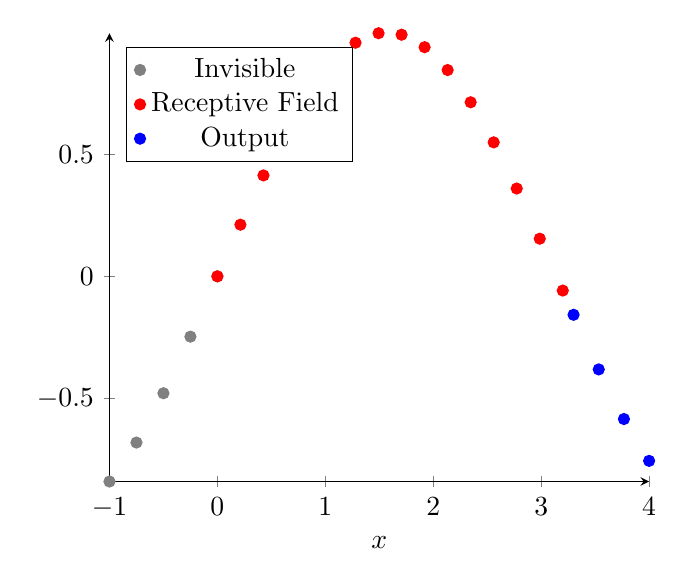
\begin{tikzpicture}
    \begin{axis}[
            axis lines = left,
            xlabel = \(x\),
            domain=-10:10,
            legend pos=north west,
        ]
        \addplot [
            domain=-1:0,
            samples=5,
            color=gray,
            only marks,
        ]
        {sin(deg(x))};
        \addlegendentry{Invisible}
        \addplot [
            domain=0:3.2,
            samples=16,
            color=red,
            only marks,
        ]
        {sin(deg(x))};
        \addlegendentry{Receptive Field}
        \addplot [
            domain=3.3:4.0,
            samples=4,
            color=blue,
            only marks,
        ]
        {sin(deg(x))};
        \addlegendentry{Output}
    \end{axis}
\end{tikzpicture}%